\section{Analysis}
\protect\label{section:tanalysis}

The performance in terms of finding objects, especially with the filters other
than \texttt{g} and \texttt{r} was not good. The various files in use were
considered in turn in an effort to improve the performance.

\subsection{Bias Files}
\protect\label{section:biasfiles}

It was noticeable that some of the pixel values, after subtraction of the master
bias files, became negative, as can be seen in both Fig. \ref{fig:exampmontage}
and \ref{fig:yearapart}. This occurs in a significant number of cases, but
particularly with the \texttt{g} filter, for example example, taking the
observations and master bias files for 5  September 2018, the total negative values shown in 
Table \ref{table:negmast} are
observed.

\begin{table}[!htbp]
\begin{center}
\begin{tabular}{lrr} \hline
Filter & Min & \% negative \\\hline
g & -27 & 28.90 \\
i & -20 & 5.42 \\
r & -19 & 5.52 \\
z & -20 & 9.90 \\
\hline
\end{tabular}
\end{center}
\caption{Negative values of pixels in image minus monthly master bias for
various filters on 5 September 2018, for all observations of \bstar, through
various visible light filters}.
\protect\label{table:negmast}
\end{table}

It is noticeable that this is worst on the \texttt{g} filter, for which some of
the best results were obtained finding images. An example of the distribution of
negative values after subtracting the appropriate master bias from the sky is
shown in Fig.
\ref{fig:negbiaseg}

\begin{figure}[!htbp]
\begin{center}
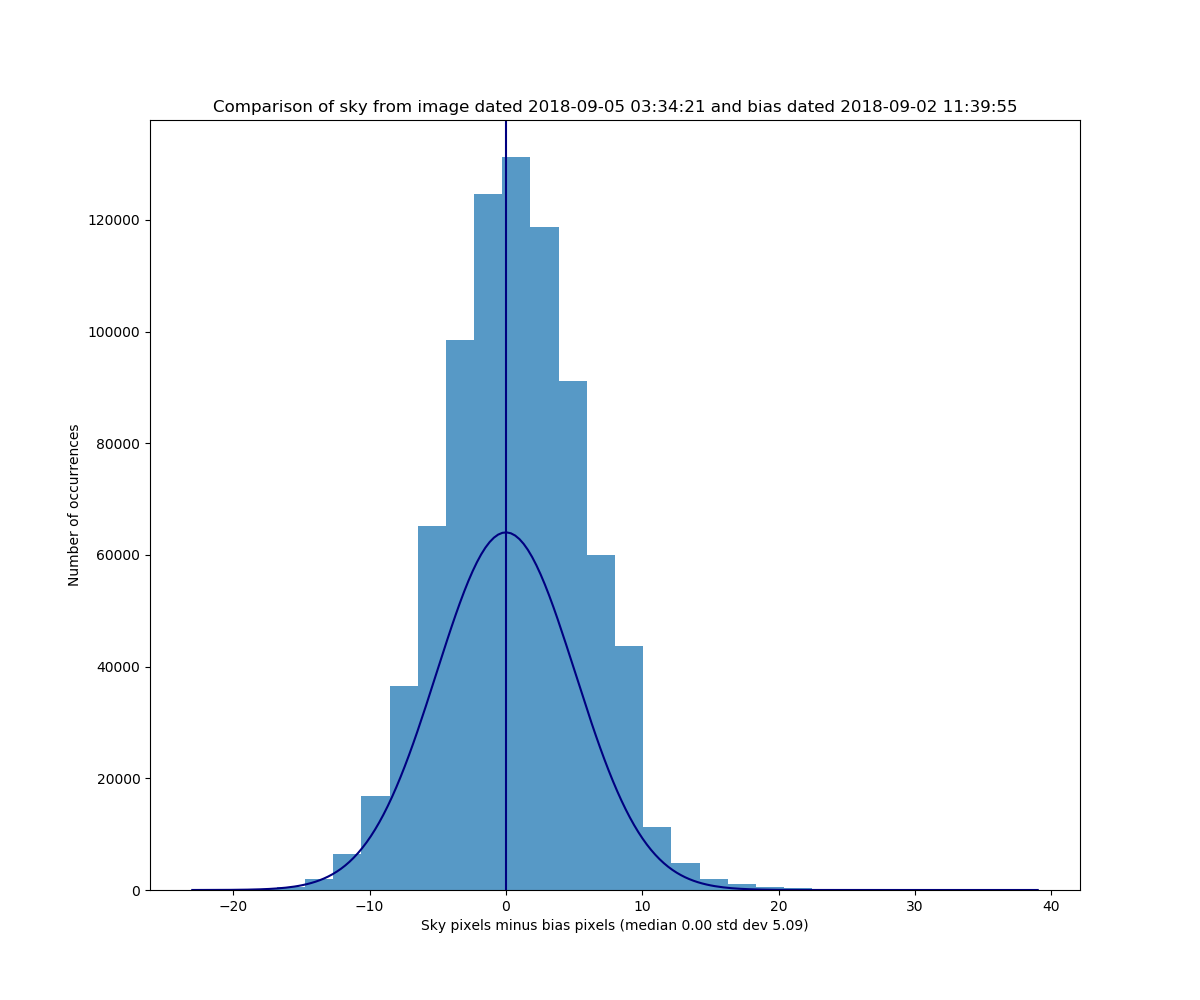
\includegraphics[scale=0.5]{images/negbiaseg.png}
\end{center}   
\caption{This shows the distribution of the values of the sky level pixels minus
the corresponding bias pixels for an observation of {\bstar} with the \texttt{g}
filter taken on on 5 September 2018 and the master bias file for September 2018.}
\protect\label{fig:negbiaseg}
\end{figure}

\subsubsection{Comparison of bias files}

The master bias files are constructed from daily bias files and it seemed
appropriate to examine these. on 5 September 2018, five daily bias files were
taken between 11:31:10 UTC and 11:37:02 UTC for each filter.

Each consecutive pair of bias files were compared against each other (after
eliminating ``spikes'') and the results set out in Fig.
\ref{fig:biascomp}.

\begin{figure}[!htbp]
\begin{center}
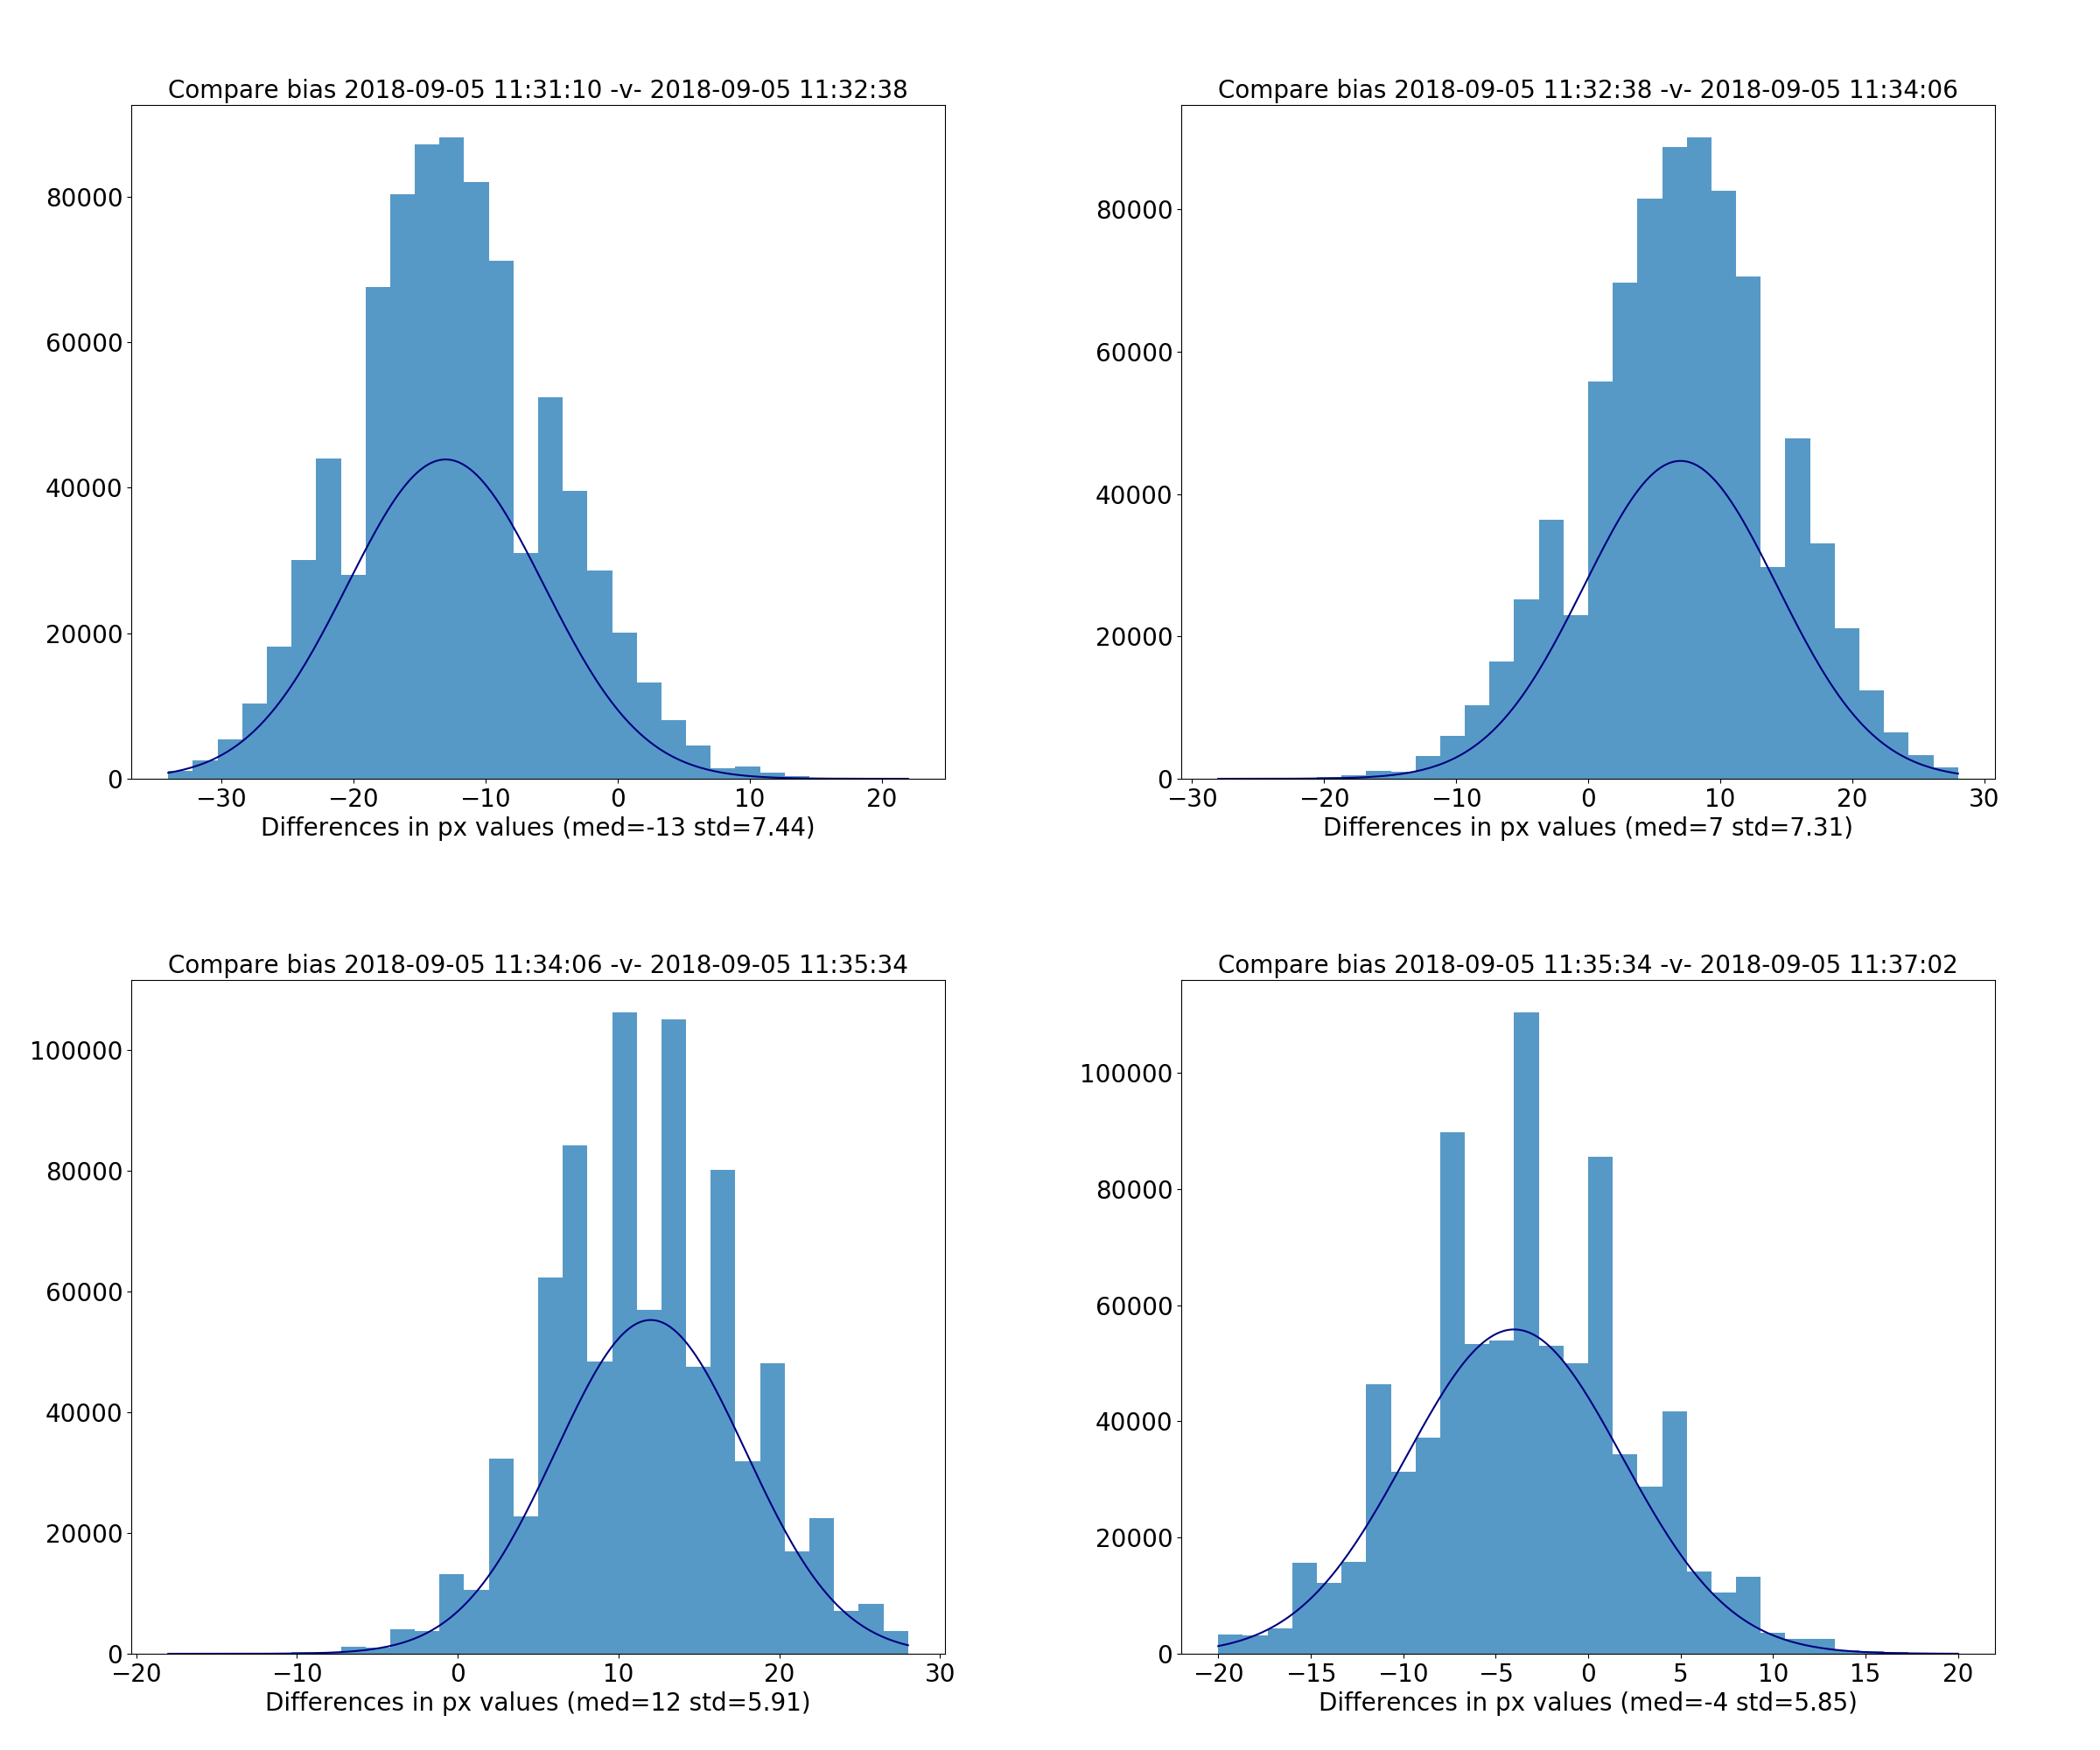
\includegraphics[scale=0.2]{images/biascomp.png}
\end{center}   
\caption{This shows the differences between successive pairs of the 5 bias
files taken on 5 September for filter \texttt{g} with times as shown in the
titles between 11:31:10 UTC and 11:37:02 UTC} \protect\label{fig:biascomp}
\end{figure}

Similar results were observed when bias files for other filters were observed,
for other dates and daily bias files several days apart were compared. The
differences would appear to be a measure of the errors in the CCD used.

A bias file was constructed by merging together all the daily bias files and the
computation shown in Fig. \ref{fig:negbiaseg} for the monthly master
bias file repeated, the result is very similar, as shown in Fig.
\ref{fig:negbiasmerg}.

\begin{figure}[!htbp]
\begin{center}
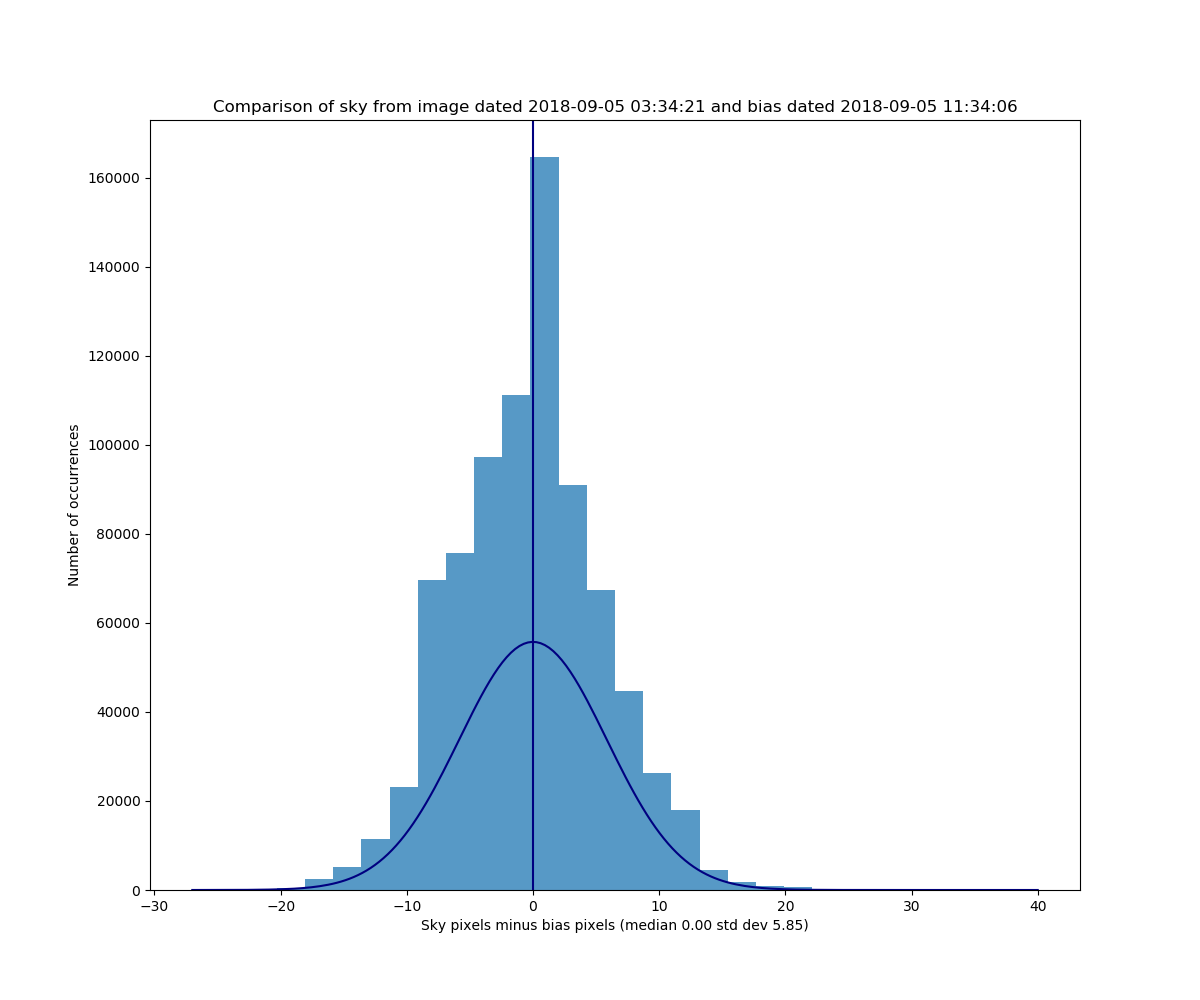
\includegraphics[scale=0.5]{images/negbiasmerg.png}
\end{center}   
\caption{This shows the distribution of the values of the sky level pixels minus
the corresponding bias pixels for an observation of {\bstar} with the \texttt{g}
filter taken on on 5 September 2018 and a bias file constructed from the bias
files taken on 5 September 2018.} \protect\label{fig:negbiasmerg}
\end{figure}

It was noticeable that, except in the case of images which were clearly
defective in other ways, the difference between the merged bias levels and the
sky levels was at most that of the standard deviation between the bias levels
shown in Fig. \ref{fig:biascomp} and was often zero as Fig.
\ref{fig:negbiaseg} and Fig. \ref{fig:negbiasmerg} show. This would suggest that
the bulk of the ``sky level'' is made up of the bias values.

\subsubsection{Hotspots or defective pixels}
\protect\label{section:hotspots}

It was noticeable that apparent findings of objects in the images consistently
showed a point source. This was particularly true of the images for the
\texttt{g} filter. It was attempted to identify such hotspots by examining the
number of bias file images in which a peak value of over 5 standard deviations appears in the same place in over 1\% of the files,
it was found that there were 1,558 such pixels in all the
\texttt{g} daily bias files, 2 in the \texttt{z} files and none in the others.
793 were in column 623, where the vertical line appears in the images and can be
seen in Fig. \ref{fig:yearapart}. No amount of adjustments to flat or bias files
can be made to overcome this consistently. It will have to be worked around by
interpolation over the areas in question.

It is unfortunate that this applies to the \texttt{g} filter as the images are
otherwise better than the others. Possibly this might give rise to ``false
positives''.

\subsubsection{Master bias files}
\protect\label{section:masterbias}

The master bias files are created by combining all the bias files for the
relevant month, using the median pixel value in each case. This is reasonable
in most cases except for the \texttt{g} filter case where there are so many
hotspots. This probably explains the high number of negative pixels after
applying the bias files noted in Table \ref{table:negmast}.


\subsection{Flat files}
\protect\label{section:flatfiles}

Two kinds of flat file are provided, a set of daily flat files for each of the
filters, typically 2 or 3 each day for each of the 4 visible light filters \textbf{g},
\textbf{i}, \textbf{r} and \textbf{z} and for gains of 1 and 4 and the monthly
master flat files, consisting of a composite of the daily flat files for the
month.

\subsubsection{Daily flat files}
\protect\label{section:dailyflatfiles}

The daily flat files, after the end of 2013, which precedes the first of the
observations, are taken with an exposure time of 1 second. Some have a gain of
4.4, in line with the gain applied to some of the other observations, but in
this report only the flat files with a gain of 1 are considered. The master flat
files are only taken from these.

Rows and columns of the image containing zero pixels were removed from the
images before analysis. (These values are replaced by \texttt{NaN} in cle master
flat files and correspond to invalid pixels.)

It was of concern that many of the daily flat files had pixels which were vary
close to saturation. in some cases they were clearly saturated, but none of the
master flat files appeared to incorporate the daily flat files with definitely
saturated pixels. In Table \ref{table:satpix} is shown the proportion of
nearly saturated pixels in flat files for each filter.

\begin{table}[!htbp]
\begin{center}
\begin{tabular}{lrrr} \hline
Filter & Flat files & Saturated & Over 50\%\\\hline
g & 3,679 & 29.49 & 22.34 \\
i & 3,679 & 32.37 & 27.43 \\
r & 3,680 & 32.66 & 28.12 \\
z & 3,680 & 0.92 & 0.60 \\\hline
Overall & 14,718 & 23.86 & 19.62\\
\hline
\end{tabular}
\end{center}
\caption{Breakdown of daily flat files by filter up to August 2019 showing
number, percentage with nearly saturated pixels present and percentage with over
50\% saturated pixels (in many cases this was over 90\% and occasionally 100\%).}
\protect\label{table:satpix}
\end{table}

\subsubsection{Linearity of CCDs}

It might be reasonable to expect that if the CCDs are linear, then the standard
deviation of the values in the daily flat files would rise in proportion to the
mean values in the daily flat files. In Fig. \ref{fig:ffcorr} is shown how this
correlates for the four filters.

\begin{figure}[!htbp]
\begin{center}
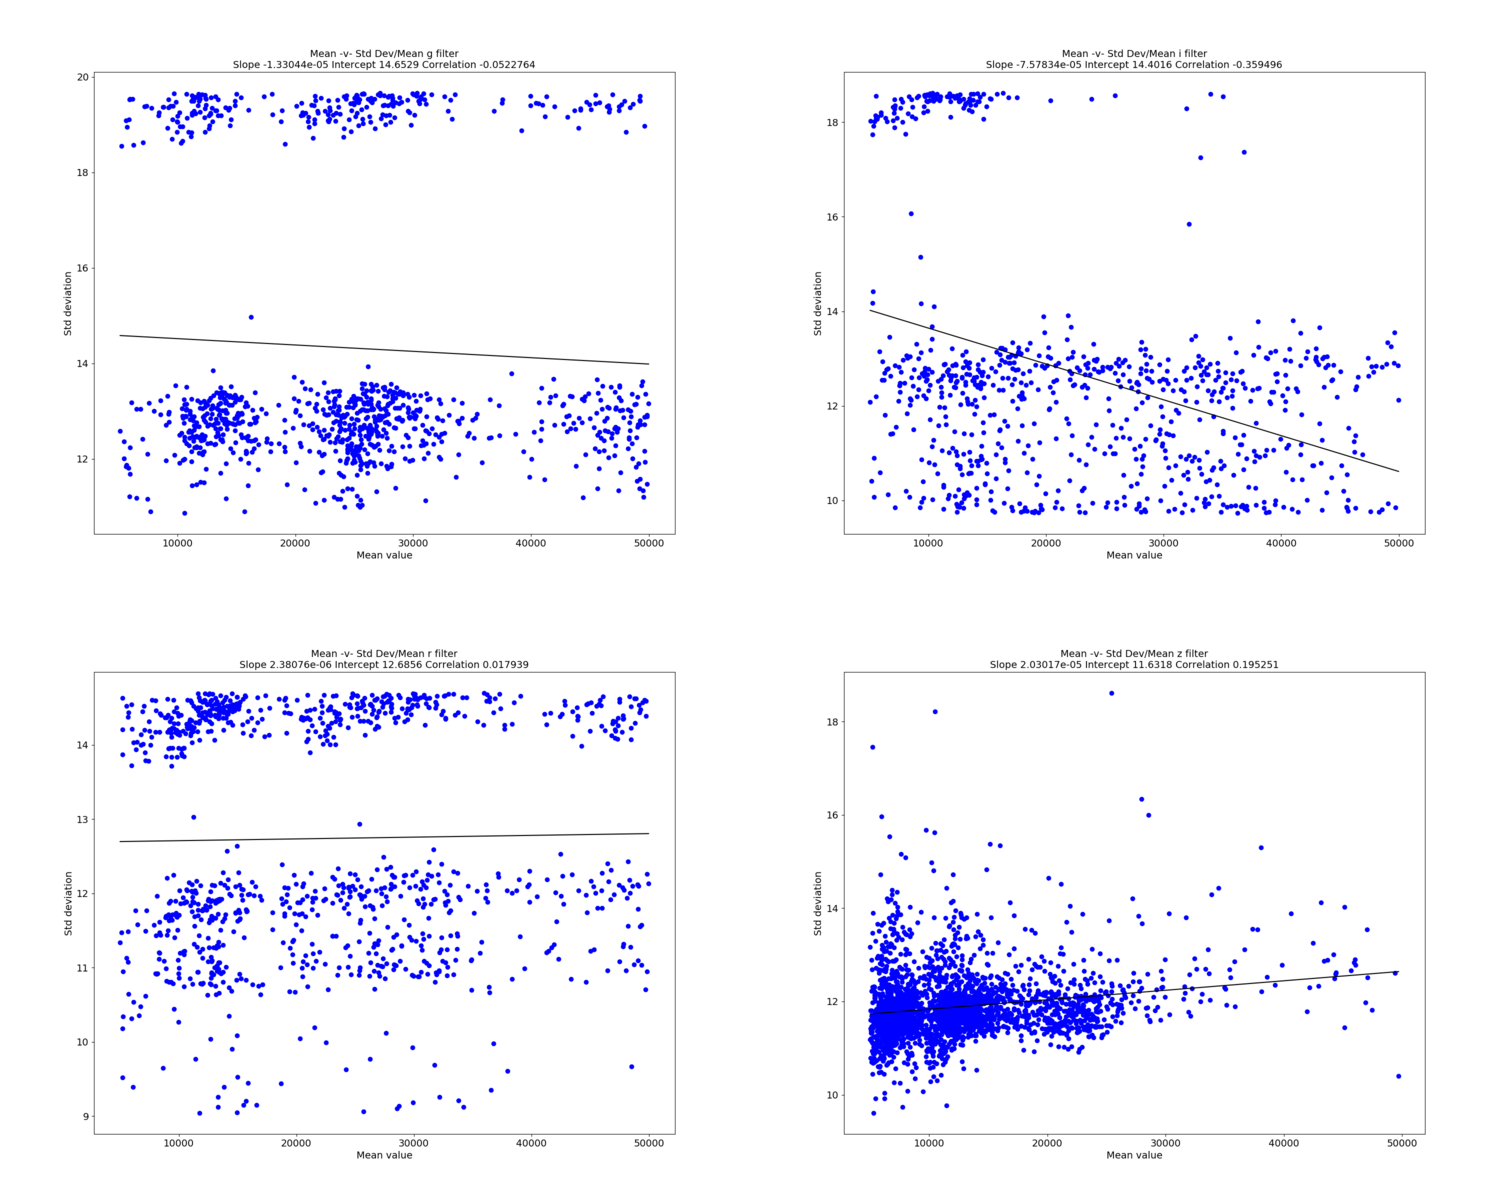
\includegraphics[scale=0.25]{images/Corr.png} \\
\end{center}   
\caption{This figure shows how the standard deviation of the values in the
daily flat files corresponds to the four filters. In the top is shown the
results for the \texttt{g} filter, the bottom left shows the \texttt{r} filter,
the top right shows the results for the \texttt{i} filter and the bottom right
shows the results for the \texttt{z} filter. The black line shows the best fit
slope in each case.}
\protect\label{fig:ffcorr}
\end{figure}

It is clear \textit{and I need another diagram to illustrate this} that
linearity drops off dramatically when the mean is below 5,000 and above 50,000.
%\
\subsubsection{Master flat files}
\protect\label{section:masterflatfiles}

The master flat files consist of median values of the incorporated daily flat
files, the header indicating which ones are considered.

Invalid pixel values are represented by \texttt{Nan} and rows and columns
containing these values are trimmed from the images, both for the flat files
themselves, and also for the corresponding bias and observations files.

The program used to create the master flat files selects daily flat files with a
mean value between 5,000 and 50,000 \textbf{and} with a negative skew and
kurtosis less than 7.\footnote{In the author's opinion the ``and'' was not
intended,}

It would appear to the author that the upper limit is too great and several
files with saturated pixels are included, using the median pixel value will
exclude these, but this creates a difficulty in that as 3 daily flat files are
taken from the sky before observations start, effectively the middle one is
taken in each case by the median.

In the author's opinion each flat file should
be normalised first and the results combined, so a procedure to create
alternative master flat files was devised. This turned out to be compromised by
the extreme values in the bias files, which made some of the pixel values
negative in the daily flat files. This primarily affected the \texttt{r} filter
(not the \texttt{g} filter as might have been expected). To complete this task
the hotspots need to be eliminated.

It was noticed that there was a computational error in the calculation of the
mean, standard deviation and other parameters in the master flat files and these
had to be discarded in any event. As the daily flat files change somewhat over
time \textit{I need to illustrate this}, reliance on a master flat file possibly
30 days removed from the observations to which it relates would seem
inappropriate and a procedure of ``rolling'' master flat files centred on the
observation dated was adopted.

\subsubsection{Accuracy}
Combination of daily bias values appears to improve the accuracy. The median
pixel value for all of the bias files for all of the filters is approximately
300 with a standard deviation of about 7 for the individual files, 3 for where
all the daily ones for a given day are merged and 1 for the master bias files.

If the counts on the actual images are considered, the following maximum pixel
values are observed, as illustrated in Table \ref{table:pmaxima}. Note that
these are extreme cases. The typical maximum is about 75\% of these.

\begin{table}[!htbp]
\begin{center}
\begin{tabular}{lr} \hline
Filter & Max pixel value \\\hline
g & 5,010 \\
i & 56,509 \\
r & 16,562 \\
z & 34,293 \\
\hline
\end{tabular}
\end{center}
\caption{Maximum pixel values in any of the observation files for 5 September
2018.}.
\protect\label{table:pmaxima}
\end{table}
\clearpage

% \subsection{Analysis of images}
% \protect\label{section:analimages}
% 
% \textbf{Please note that since I realised that the master flat files are not
% normalised as Luciano told me I'll have to redo all this. The results within
% each month are consistent but not with other months. Also with the flat files
% properly normalised some of the images will have greater contrast.}
% 
% \subsubsection{Intensity comparison}
% \protect\label{section:intcomp}
% 
% As a first attempt to study the data, the ADU count was taken, specifically the
% net after applying the flat and bias files of the target in all the images in which it was available.
% The target was found in all of the images, apart from in a few of the
% \textbf{g}, \textbf{i} and \textbf{r} visible light filters,
%, as shown in Table
%\ref{table:occtb} below.

%Plotting light curves of the intensities obtained in this way yields Fig.
% \ref{fig:allall}.
%Binning the intensities together into a single day gave
%Fig. \ref{fig:allbin}, the error bars indicate the spread over a single day.

%I plotted
%periodograms, as shown in Fig. \ref{fig:pgrams}. Despite the crudeness of the
%data, it is noticeable that there are peaks close to the rotation periods of
% the order of 150 days referred to in \citet{suarezmascareno15} and \citet{toledopadron18}.

% \begin{figure}[!htbp]
% \begin{center}
% 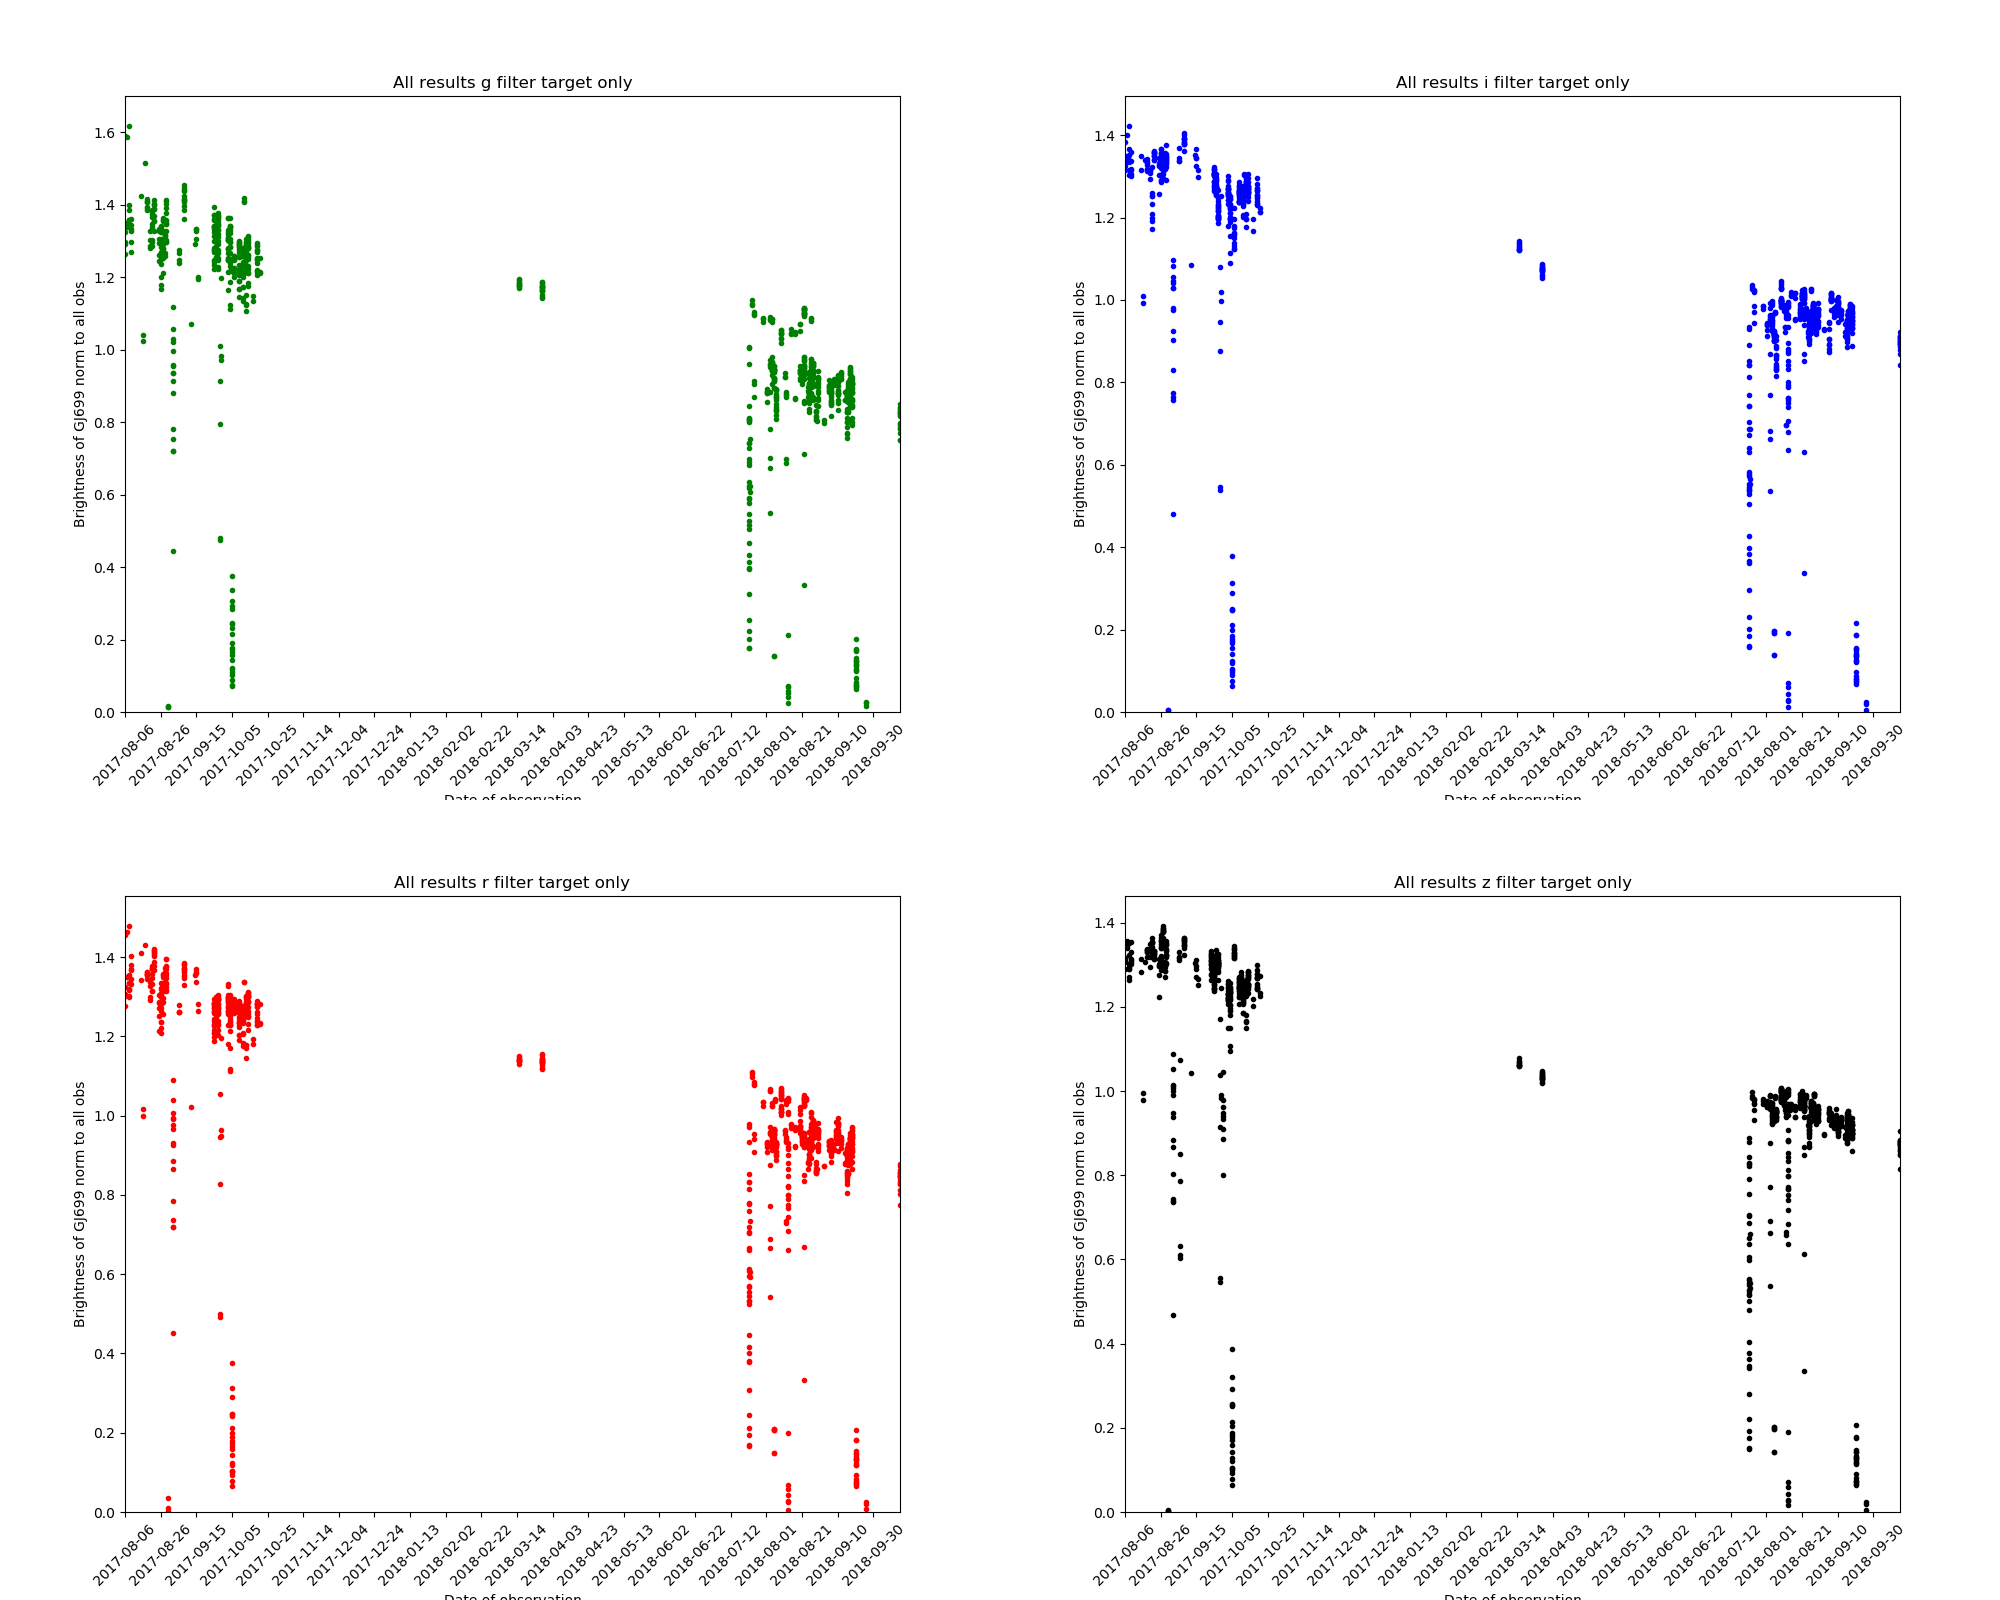
\includegraphics[scale=0.25]{images/allall.png} \\
% \end{center}   
% \caption{This shows the flux for the target, \bstar, for each of the four visible light filters. This takes the total
%   ADU count only}
%   \protect\label{fig:allall}
% \end{figure}
% 
% \begin{figure}[!htbp]
% \begin{center}
% 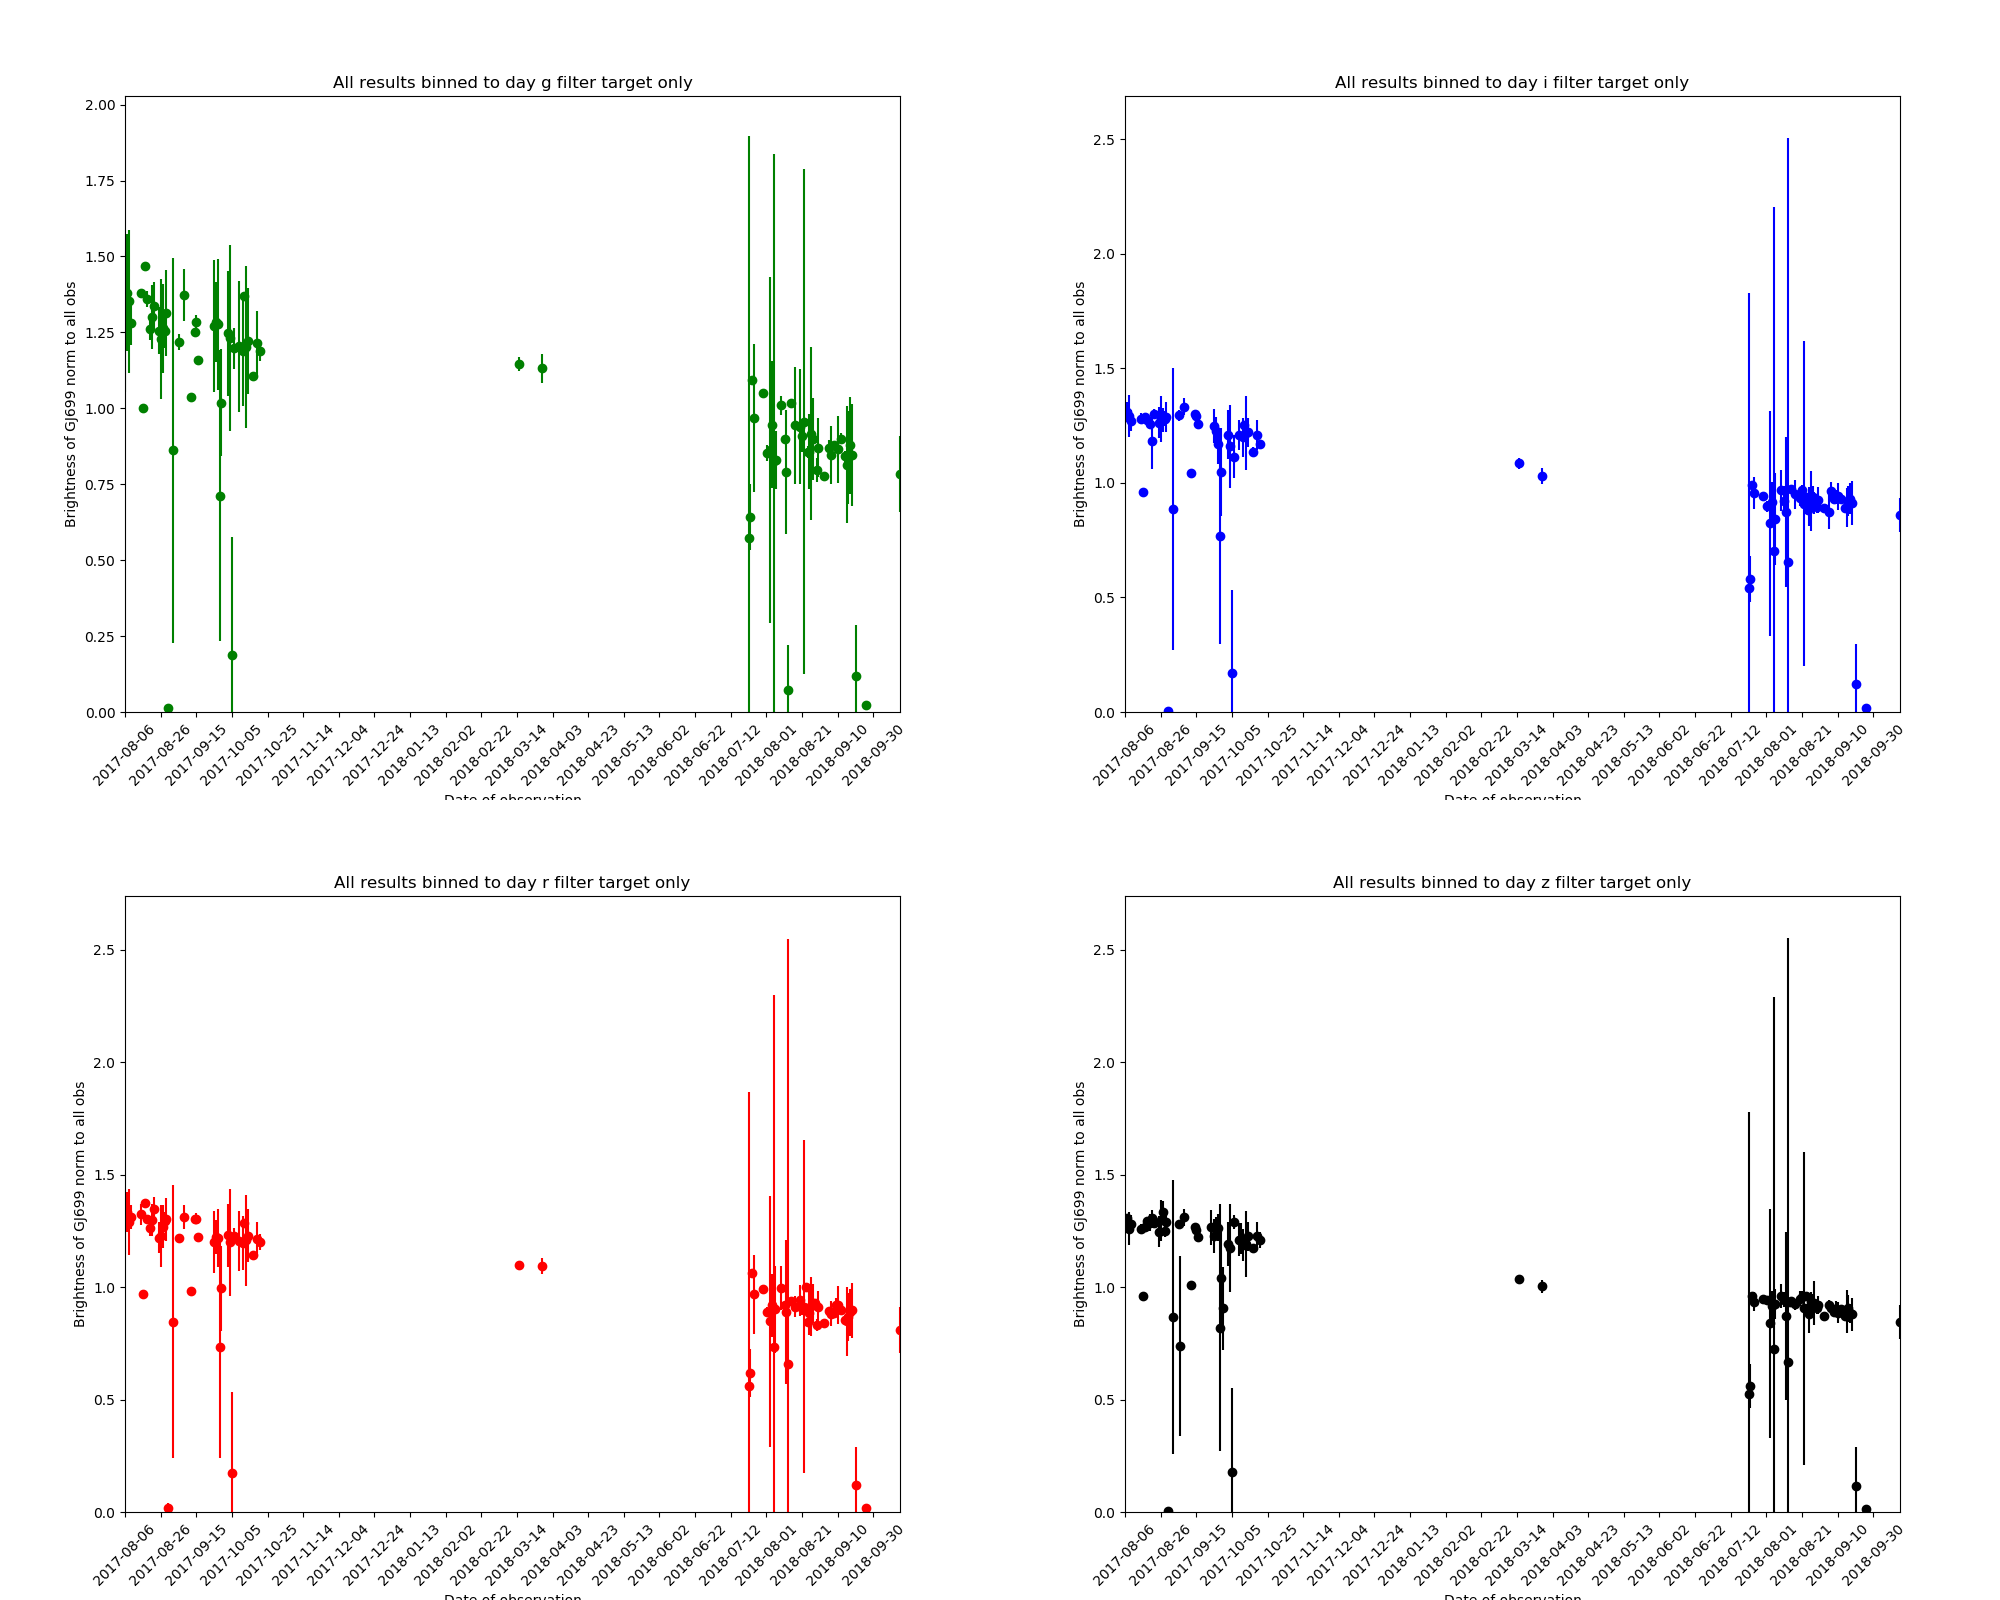
\includegraphics[scale=0.25]{images/allbin.png} \\
% \end{center}   
% \caption{This shows the flux for the target, \bstar, for each of the four visible light filters and binned to a single day. Error bars are show to indicate the spread of intensities over a single day.}
%   \protect\label{fig:allbin}
% \end{figure}

%\begin{figure}[!htbp]
%\begin{center}
%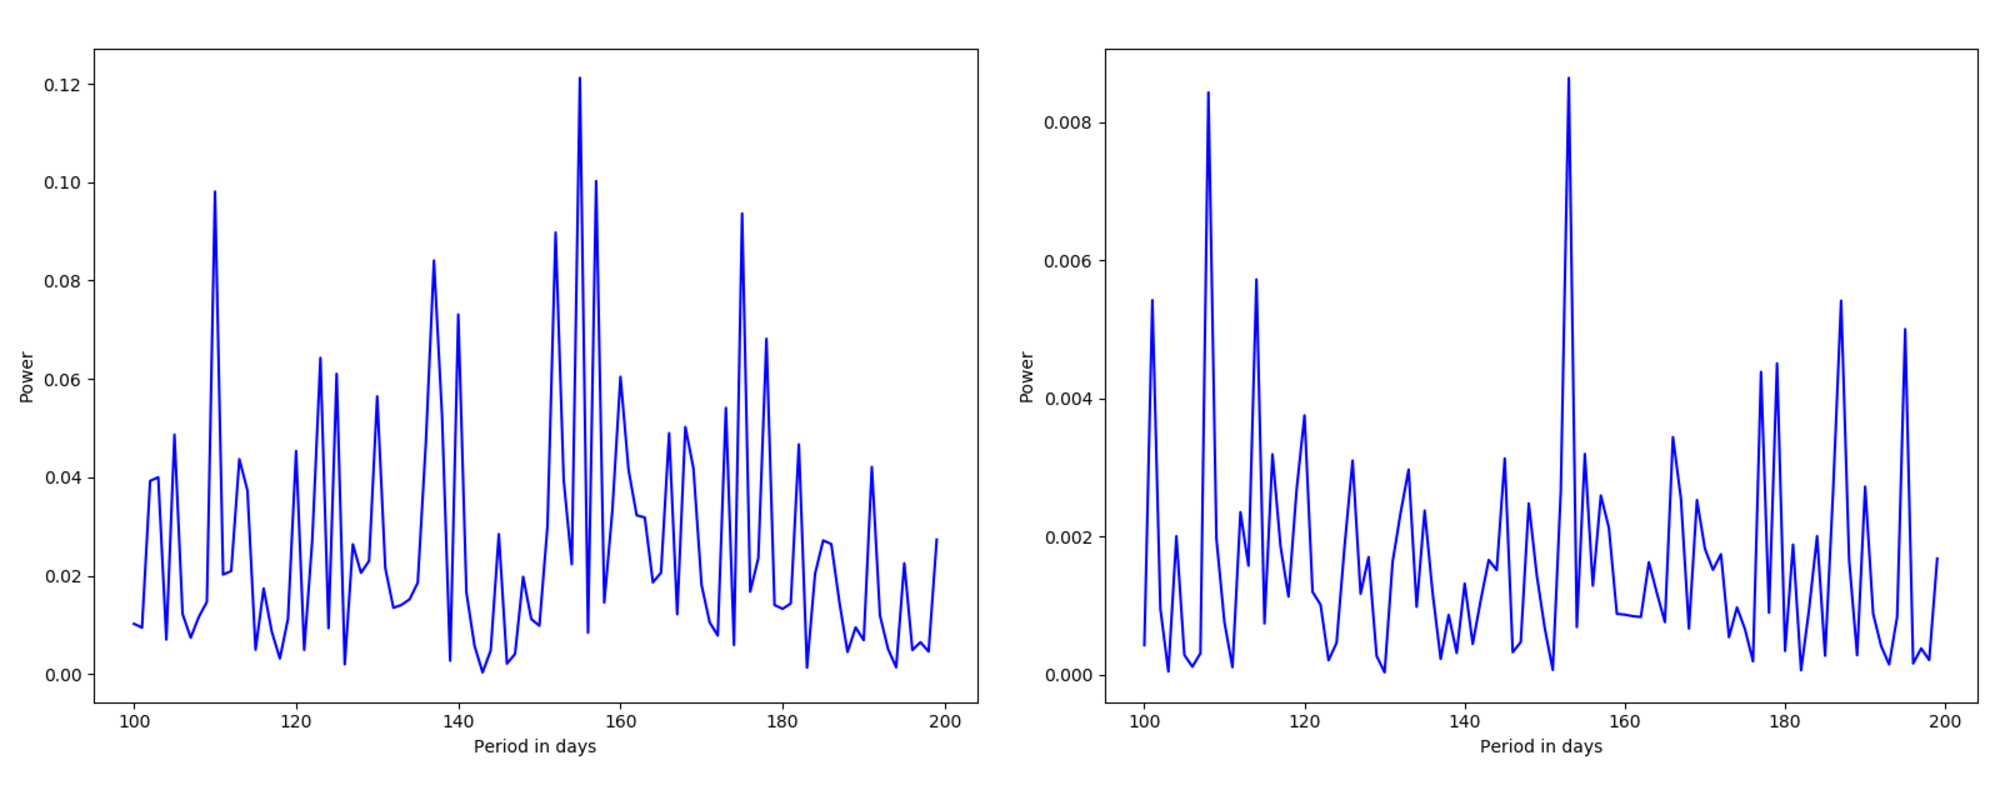
\includegraphics[scale=0.25]{images/pgrambunb.png} \\
%\end{center}   
%\caption{This displays periodograms derived from the binned (Fig.
% \ref{fig:allbin}) and unbinned (Fig. \ref{fig:allall}) light curves for the \textbf{r} filter.}
%  \protect\label{fig:pgrams}
%\end{figure}

% It is accepted that this initial treatment is crude. Serious work needs to be done on correction for air mass,
% which for a few observations, where they are spread over a period of several hours,
% can be quite large, and to more accurately discard as unacceptable images with large or very variable sky levels.
% There are some currently inexplicable variations, for
% example the to images in Fig. \ref{fig:tyeg} give radically different ADU counts despite being taken two minutes apart
% with same exposure time and other parameters.
% 
% \begin{figure}[!htbp]
% \begin{center}
% 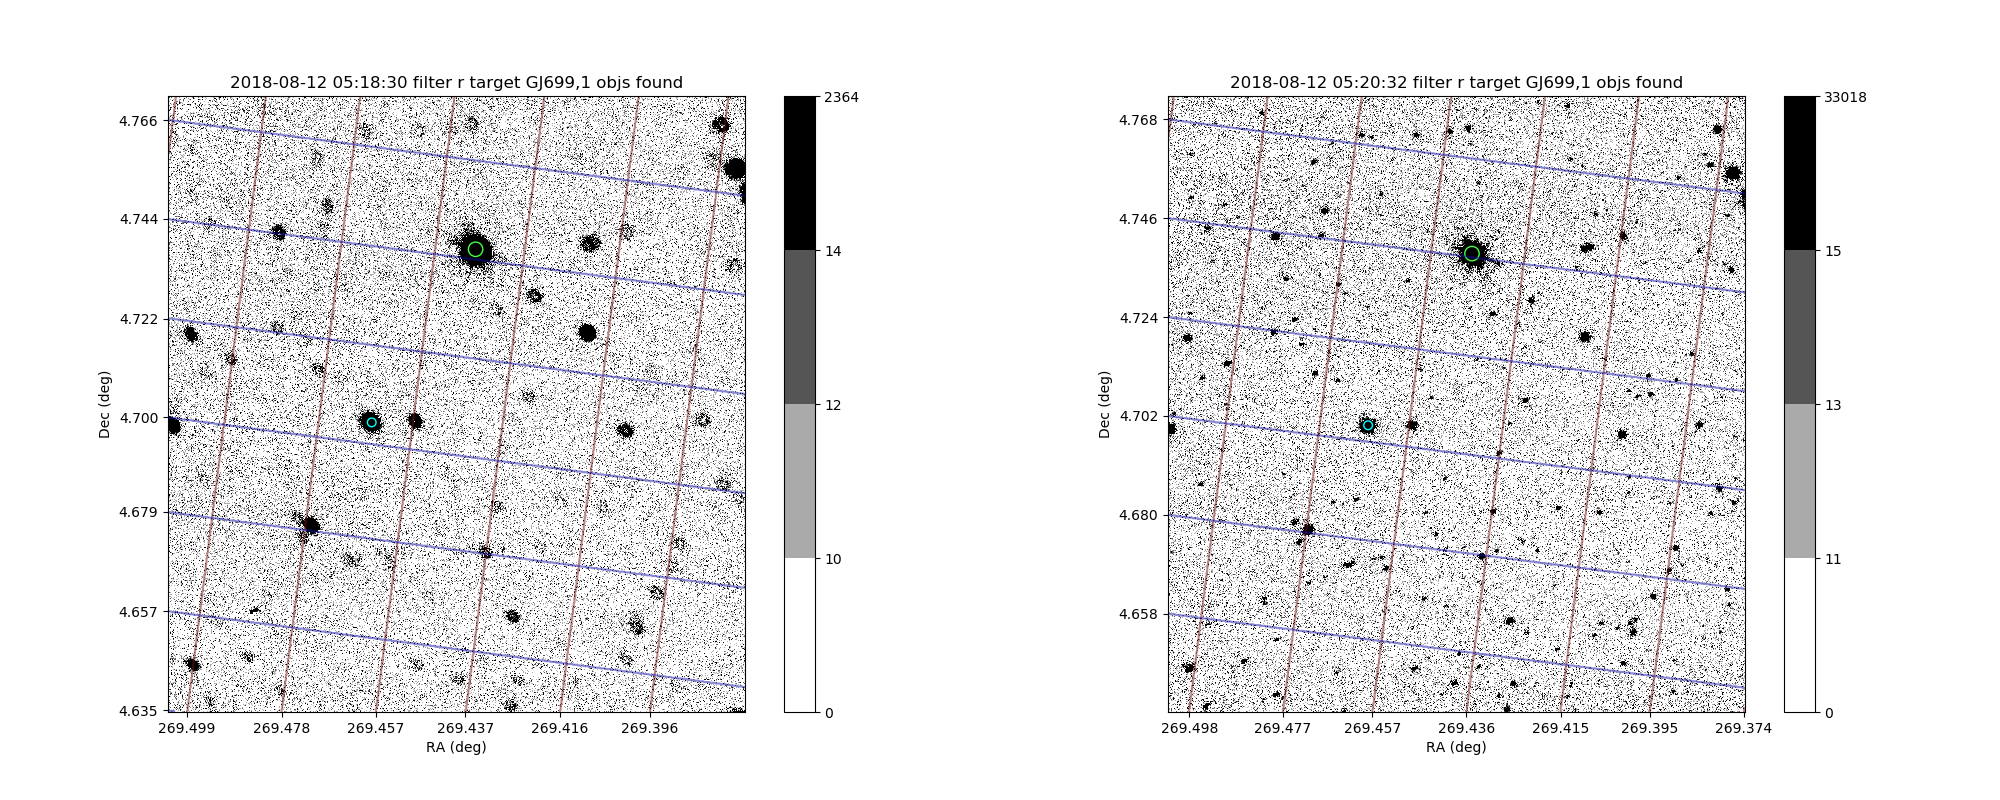
\includegraphics[scale=0.25]{images/tyeg.png}
% \end{center}   
% \caption{These images show an example of where 2 images taken 2 minutes apart with the same exposure time gave different flux values.}
%   \protect\label{fig:tyeg}
% \end{figure}
% 
% \subsubsection{Reference Stars}
% \protect\label{section:refstars}
% 
% Rather than relying on the ``raw'' flux from the target star itself, it was
% considered that an approach based on identified reference stars found in a
% significant number of images.
% Ideally these should be as many as possible to ``smooth'' out errors and variations on the reference star. 
% Byy taking the ratio of the target star ADU count to the sum of the reference
% star ADUs, then we can hope to achieve results for intensity with the factors such air mass corrections factored out, This
% approach was taken in \citet{berry11} and would seem to involve least work, provided sufficient reference stars are
% consistently found.
% 
% The algoritm used to find objects was first to locate the target (there was
% usually a certain amount of error in the coordinates of the images) and then
% find prefeviously-known reference objects. The criterion for finding objects was to look for groups of pixels within a
% given scan aperture whose mean count was a given number of standard deviations
% (intially 3) from that of the sky level. If the result appeared to be one of
% the objects known already, the given reference object was deemed to have been
% found.

% In all cases the brightest objects were found in Simbad, 2MASS and SDSS
% to find objects in the vicinity of \bstar, obtaining the following stars as shown in Table \ref{table:reftimesfound}.
% Of the stars there, the types are unavailable apart from the most-frequently occurring one of
% TYC425-262-1, which is an A3V star (this is also reported as the most frequently found reference star in \citet{berry11}).
% 
% \begin{table}[!htbp]
% \begin{center}
% \begin{tabular}{llr} \hline
% Number & Object & Times found \\\hline
% 1 & TYC425-262-1 & 5,277 \\
% 2 & SDSS1237671695527248969 & 3,408 \\
% 3 & 2MASSJ17574653+0447466 & 3,297 \\
% 4 & SDSS1237668573088841773 & 840 \\
% 5 & TYC425-223-1 & 369 \\
% 6 & SDSS1237671695527249415 & 15 \\
% \hline
% \end{tabular}
% \end{center}
% \caption{This lists the identified reference objects near to {\bstar} and the number of times found in the available
%   data. Note that this data relates to images up to the end of October 2018.}
% \protect\label{table:reftimesfound}
% \end{table}
% 
% I decided to consider only the first 3 reference objects, which are labelled 1, 2 and 3 for convenience in the
% remainder of this report, as the appearances of the others were too infrequent to render them worthwhile.
% 
% \subsection{Classification of results}
% \protect\label{section:classresults}
% 
% The images presented challenges in various respects. The visible light images are all at different orientations and with
% the target in different places in the image, so not all the reference stars appear in all of the images. In some cases
% the reference stars are just not bright enough to rise sufficiently above the sky level.
% 
% \begin{table}[!htbp]
% \begin{center}
% \begin{tabular}{lrrrr}
% &Filter g&Filter i&Filter r&Filter z\\\hline
% Target not found&167&80&105&0\\
% No ref objs found & 84 & 1,003 & 53 & 1,085 \\\hline
% Obj 1 (with or without others) & 834 & 0 & 925 & 0 \\
% Obj 2 (with or without others) & 561 & 1 & 574 & 0 \\
% Obj 3 (with or without others& 526 & 0 & 573 & 0 \\
% Obj 1 only & 43 & 0 & 100 & 0 \\
% Obj 2 only & 0 & 1 & 1 & 0 \\
% Obj 3 only & 0 & 0 & 0 & 0 \\
% Objs 1 and 2 (with or without 3) & 561 & 0 & 573 & 0 \\
% Objs 1 and 3 (with or without 2) & 526 & 0 & 573 & 0 \\
% Objs 2 and 3 (with or without 1) & 296 & 0 & 321 & 0 \\
% Objs 1 and 2 only & 265 & 0 & 252 & 0 \\
% Objs 1 and 3 only & 230 & 0 & 252 & 0 \\
% Objs 2 and 3 only & 0 & 0 & 0 & 0 \\
% Objs 1,2 and 3 & 296 & 0 & 321 & 0 \\
% \hline
% \end{tabular}
% \end{center}
% \caption{This table shows the occurrences of the 3 main reference objects in each of the observations with or without
%   the others. The infrared images were omitted as no reference objects were found in any of them. Note however the lack
%   of occurrences of reference objects in the \textbf{i} and \textbf{z} filter images.}
% \protect\label{table:occtb}
% \end{table}
% 
% \subsection{Results from reference object comparisons}
% \protect\label{section:refobjres}
% 
% Repeating the light curve plots from Section \ref{section:intcomp}, this time as the ratio of the ADU count of the
% target to the sum of the first three reference objects, Fig.  \ref{fig:allref123} and Fig. \ref{fig:allref123bin} show
% the light curves for the \textbf{r} and \textbf{g} filters. Also shown in Fig. \ref{fig:ls123both} are periodograms
% derived from these light curves. Also shown in Fig \ref{fig:allref1}, Fig. \ref{fig:allref1bin} and Fig. \ref{fig:ls1both}
% are the corresponding results taking into account only the brightest of the reference objects, TYC425-262-1.
% 
% \begin{figure}[!htbp]
% \begin{center}
% 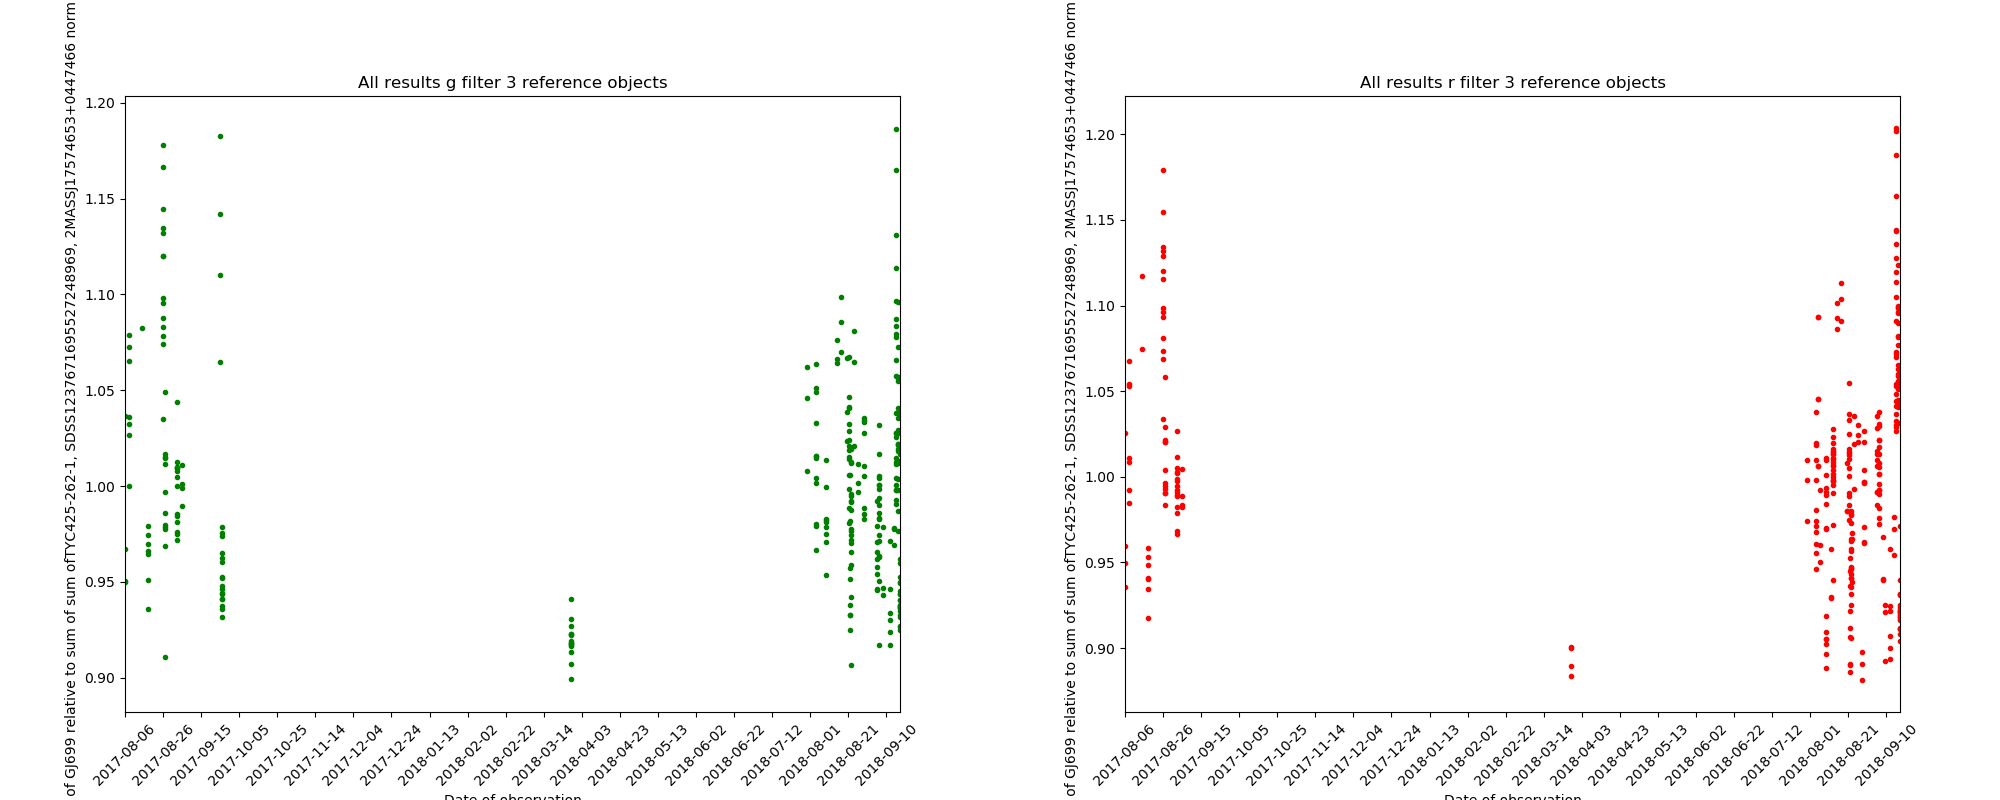
\includegraphics[scale=0.25]{images/allref123.png}
% \end{center}   
% \caption{This shows the ratio of the flux for the target, \bstar, to the 3 main reference objects for the \textbf{g} and
% \textbf{r} filters, plotted as green and red respectively.}
%   \protect\label{fig:allref123}
% \end{figure}
% 
% \begin{figure}[!htbp]
% \begin{center}
% 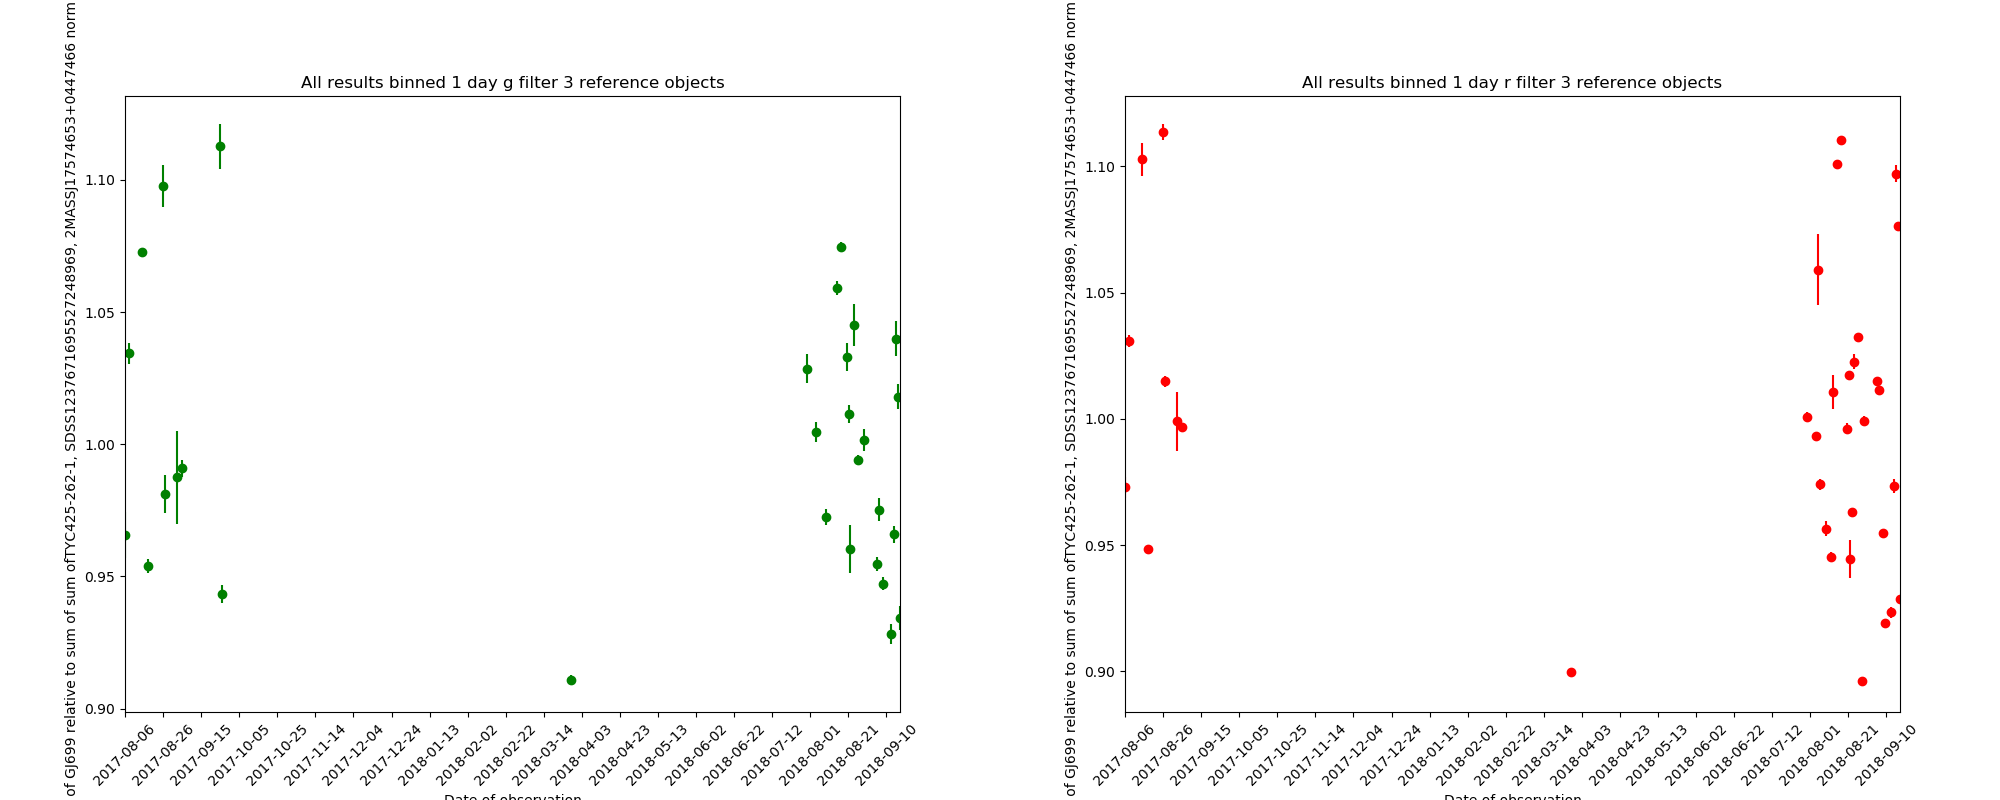
\includegraphics[scale=0.25]{images/allref123bin.png}
% \end{center}   
% \caption{This shows the ratio of the flux for the target, \bstar, to the 3 main reference objects as per Fig. \ref{fig:allref123} and binned to 1 day.}
%   \protect\label{fig:allref123bin}
% \end{figure}
% 
% \begin{figure}[!htbp]
% \begin{center}
% 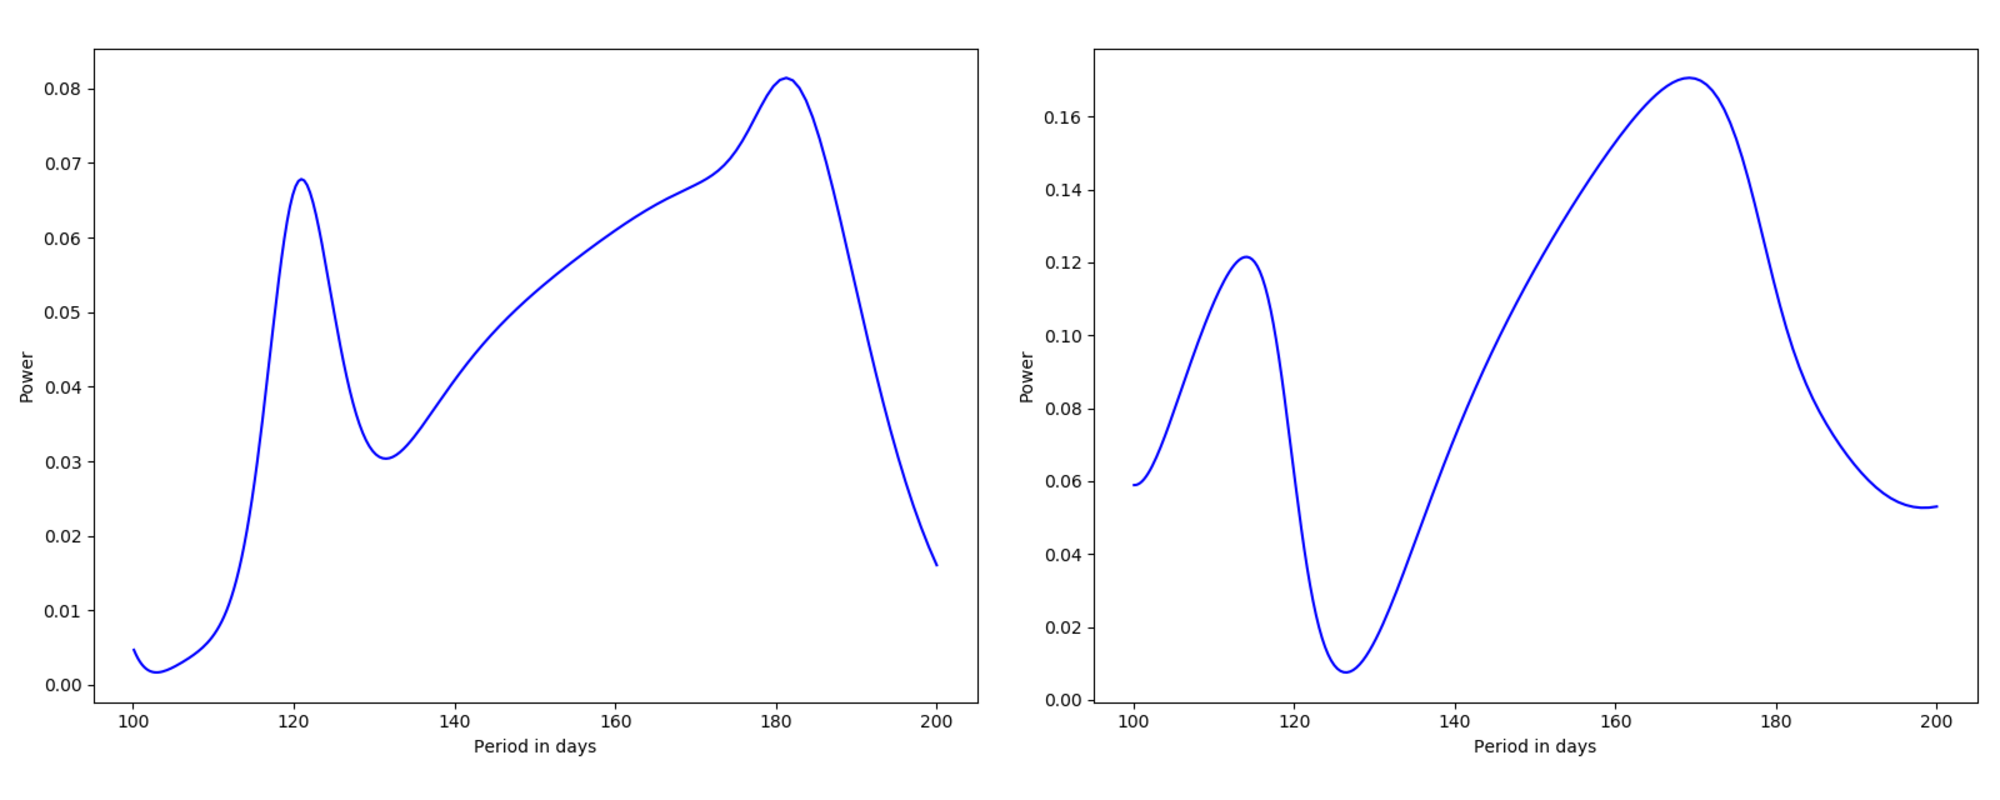
\includegraphics[scale=0.25]{images/ls123both.png}
% \end{center}   
% \caption{Periodograms obtained from Fig. \ref{fig:allref123}, left panel and Fig. \ref{fig:allref123bin} in right
%   panel. Only the \textbf{g} filter was used in this plot, the one from the \textbf{r} filter being almost identical.}
%   \protect\label{fig:ls123both}
% \end{figure}
% 
% \begin{figure}[!htbp]
% \begin{center}
% 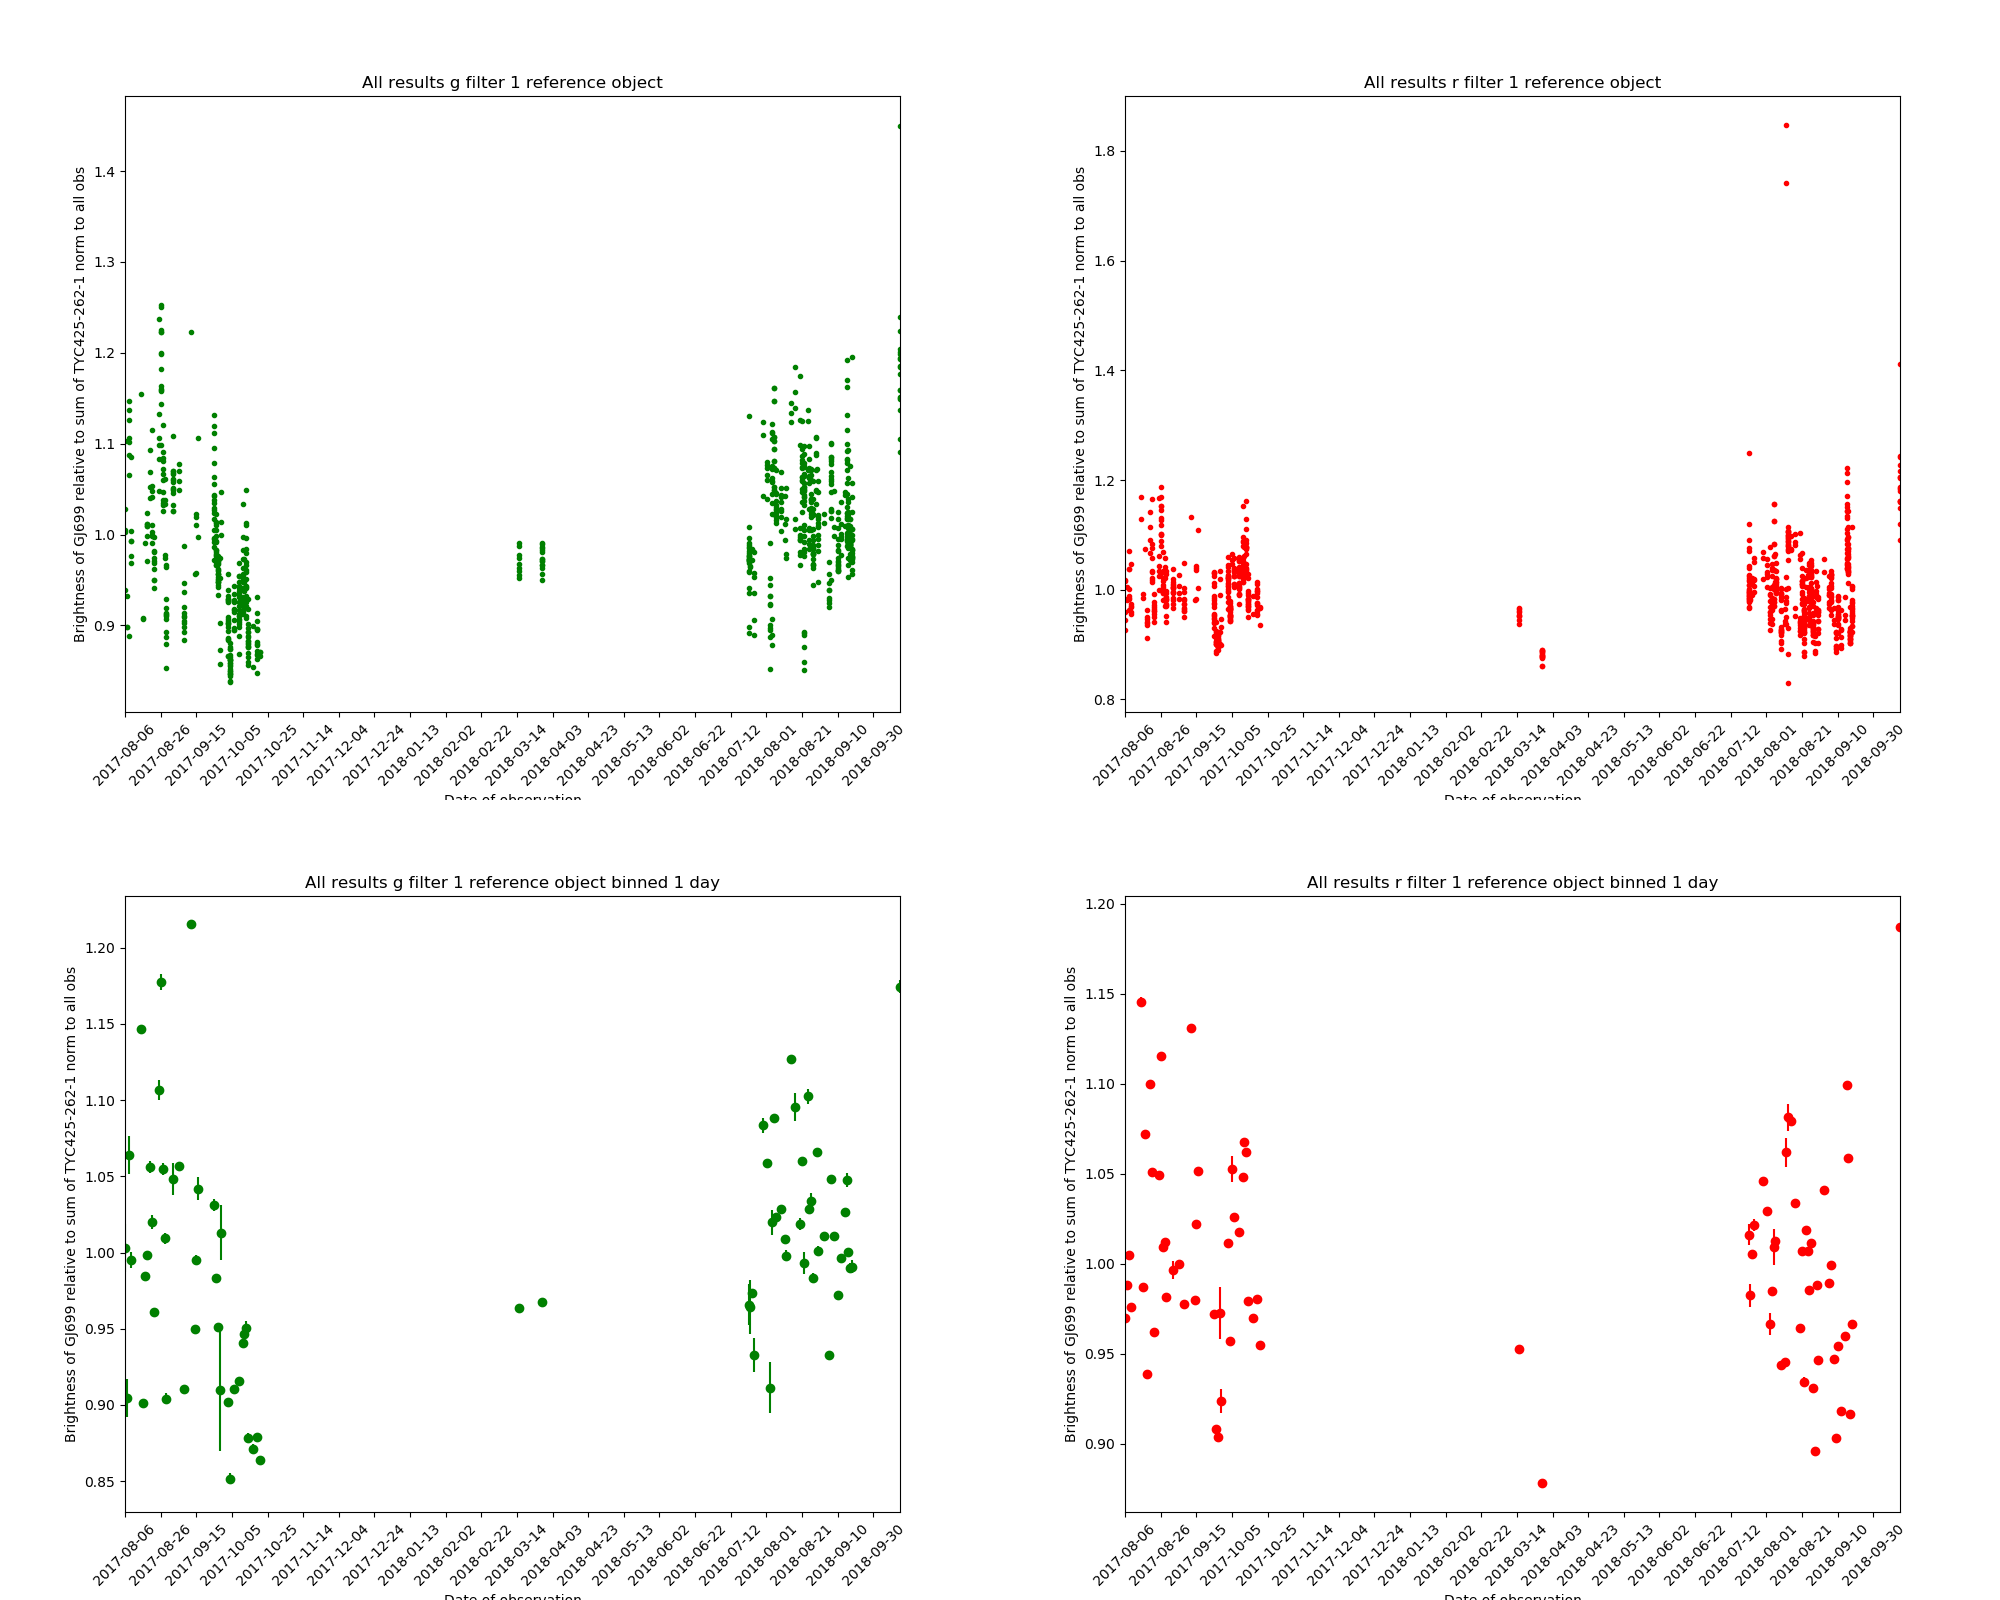
\includegraphics[scale=0.25]{images/allref1.png}
% \end{center}   
% \caption{This shows the ratio of the flux for the target, \bstar, to the strongest of the reference objects, TYC425-262-1.}
%   \protect\label{fig:allref1}
% \end{figure}
% 
% \begin{figure}[!htbp]
% \begin{center}
% 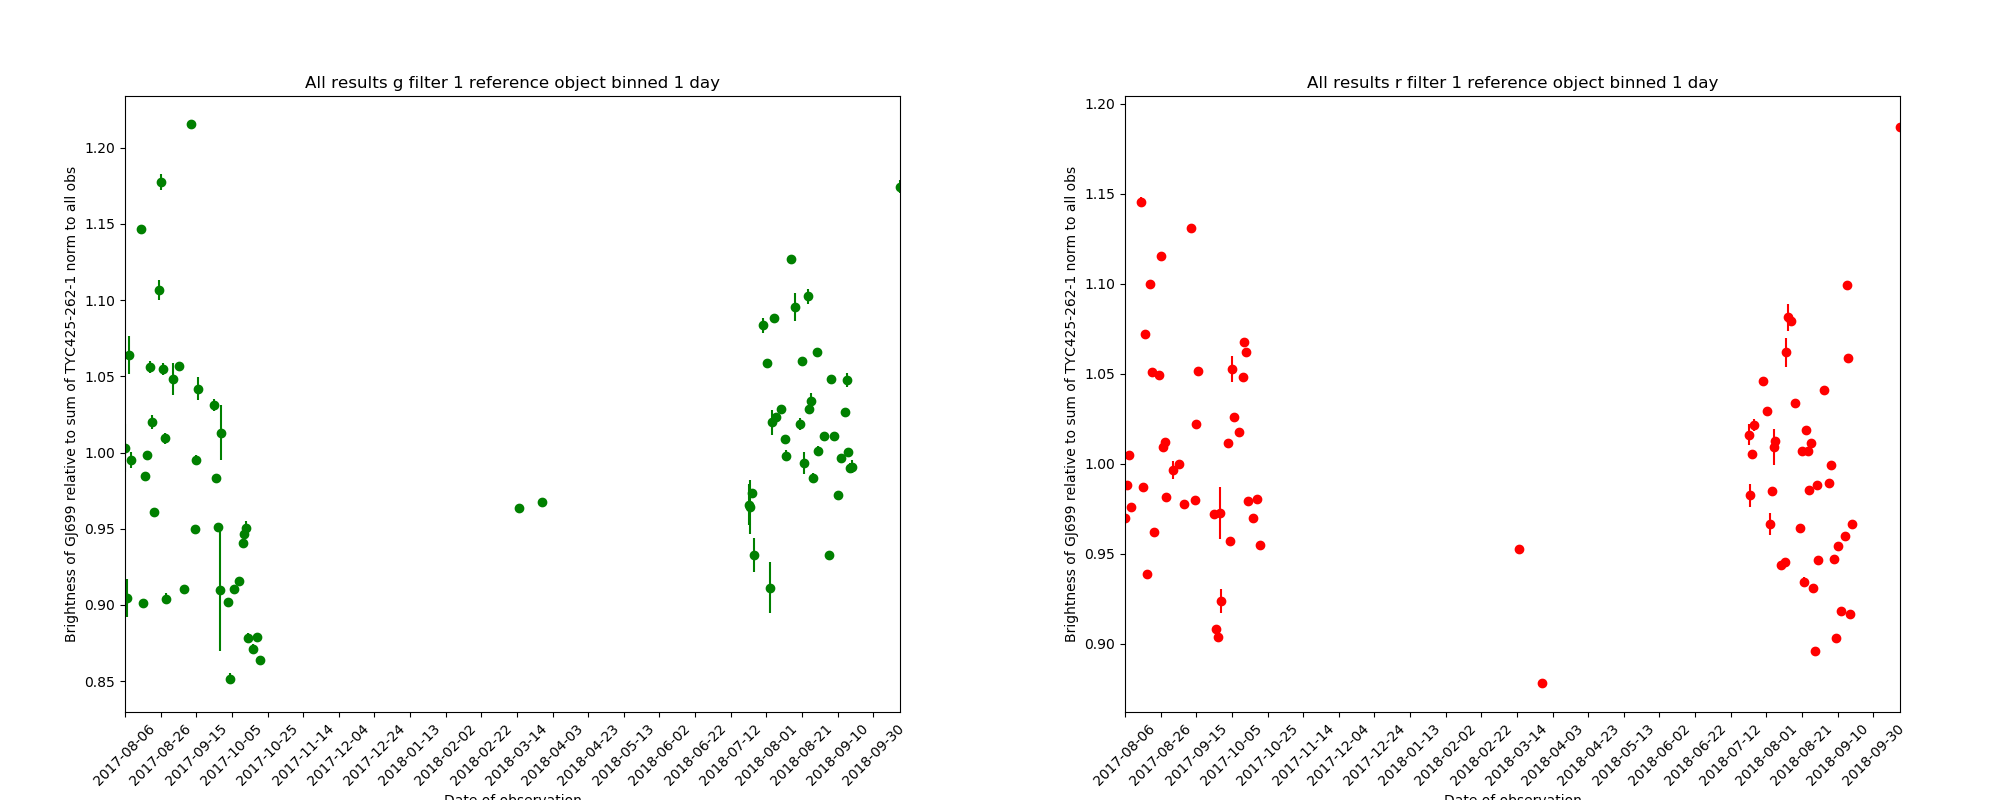
\includegraphics[scale=0.25]{images/allref1bin.png}
% \end{center}   
% \caption{This shows the ratio of the flux for the target, \bstar, to the strongest of the reference objects,
%   TYC425-262-1 per Fig. \ref{fig:allref1} and binned to 1 day.}
%   \protect\label{fig:allref1bin}
% \end{figure}
% 
% \begin{figure}[!htbp]
% \begin{center}
% 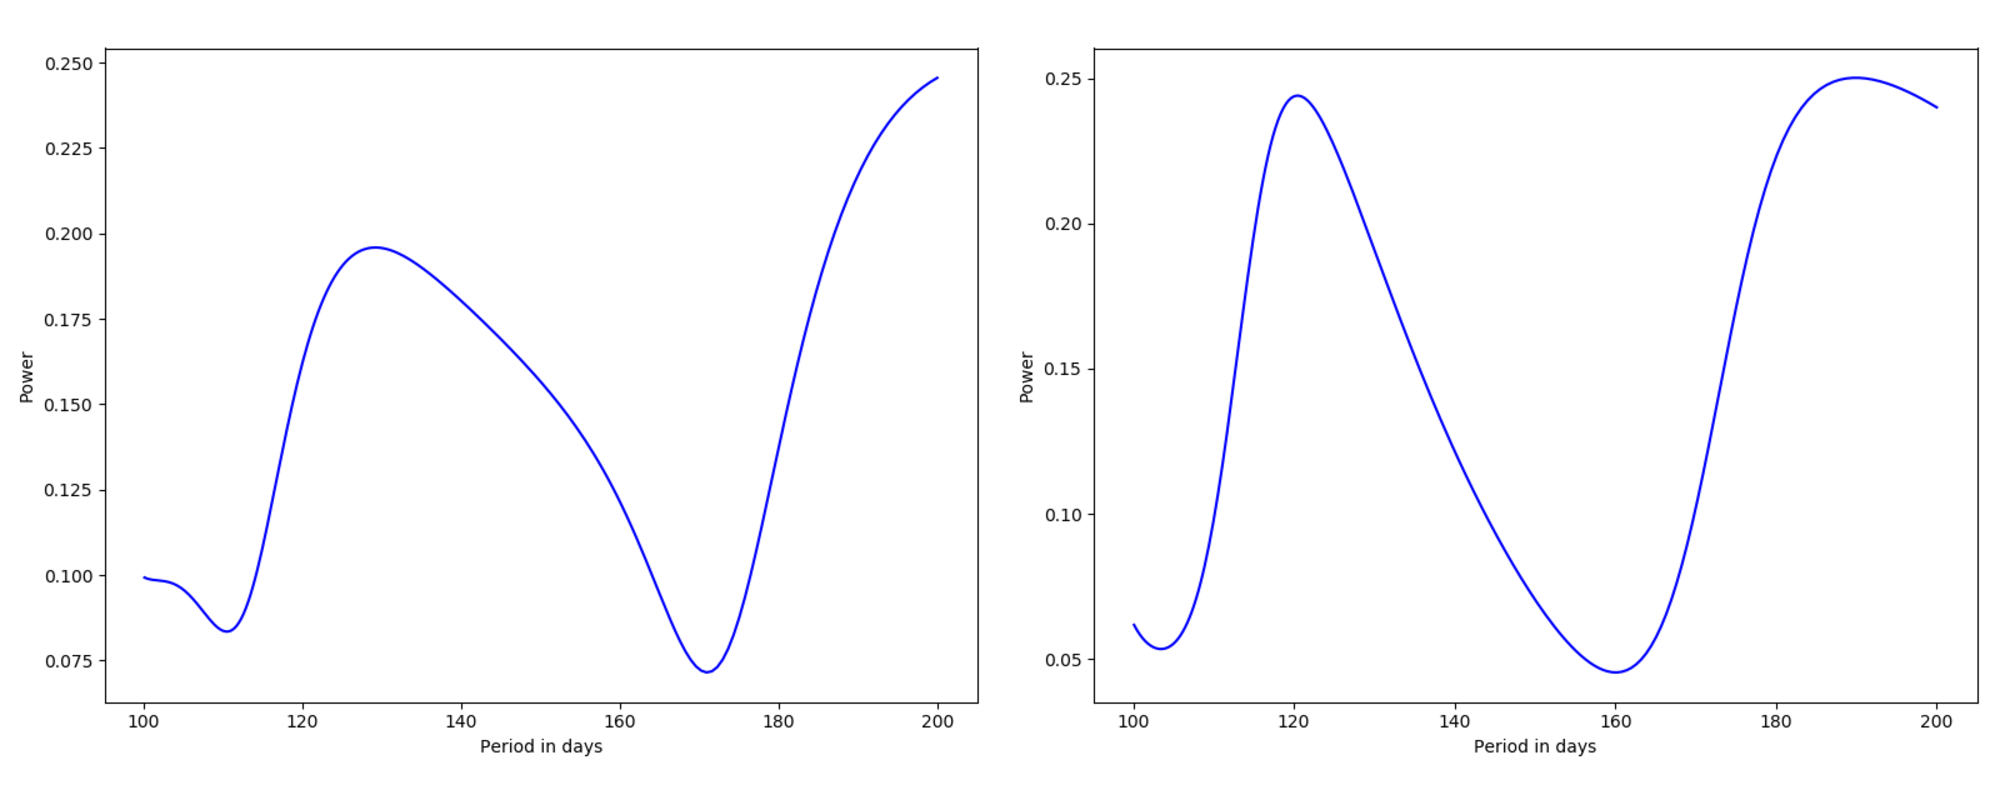
\includegraphics[scale=0.25]{images/ls1both.png}
% \end{center}   
% \caption{Periodograms obtained from Fig. \ref{fig:allref1}, left panel and Fig. \ref{fig:allref1bin} in right
%   panel. Only the \textbf{g} filter was used in this plot, the one from the \textbf{r} filter being almost identical.}
% \protect\label{fig:ls1both}
% \end{figure}
% \clearpage

